The $\crele$ is enriched in $\wenuplusjets$ processes and is used in the
computation of the V + jets background contamination in the signal
region. Besides cuts from B to H as defined in \cref{sec:event-selection-1},
this region has the following specific selections:
\begin{itemize}
\item The online trigger is required to select events with exactly one electron
  in the final state.
\item The baseline muons are vetoed.
\item In order to exclude the crack region (see \cref{sec:atlas-tilecal}),
  exactly one baseline electron with $\pt > 30$~GeV and $|\eta| > 1.52$ or
  $|\eta| < 1.37$ is selected.
\item A tight isolation criteria as defined in \cref{sec:electrons} for the
  selected electrons is required.
\item The transverse mass of the $\met - e$ system is required to be
  $30 < m_\mathrm{\, T} < 100$~GeV, compatible with a $W \rightarrow e \nu$
  process.
\item The events must satisfy: $\met/\sqrt{H_\mathrm{\, T}} > 5$~GeV$^{1/2}$
  ($\met$ \emph{significance}) where $H_\mathrm{T}$ is the scalar sum of the
  $\pt$ of the electron and the jets in the final state.
\end{itemize}
The single electron trigger, the veto of electrons in the crack region, the
tighter isolation and the $\met$ significance criteria all aim at reducing the
multi-jet contribution in this region. In order to apply the theory corrections
on V + jets discussed in \cref{sec:corrections-vjets} the \glspl{cr} have to be
enriched in $W$ + jets events thus requiring a uniform cut definition between
this control region and the $\crwmn$. For this reason in this version of the
analysis the cut on the transverse mass is
introduced. \cref{fig:ele_cr_plots_2016} shows the $\met$ and leading jet $\pt$
distribution of the $\crele$ control region. There is a good agreement within
uncertainties between data and \gls{mc}.
\begin{figure}[!th]
  \centering
  \begin{subfigure}[t]{.48\linewidth}
    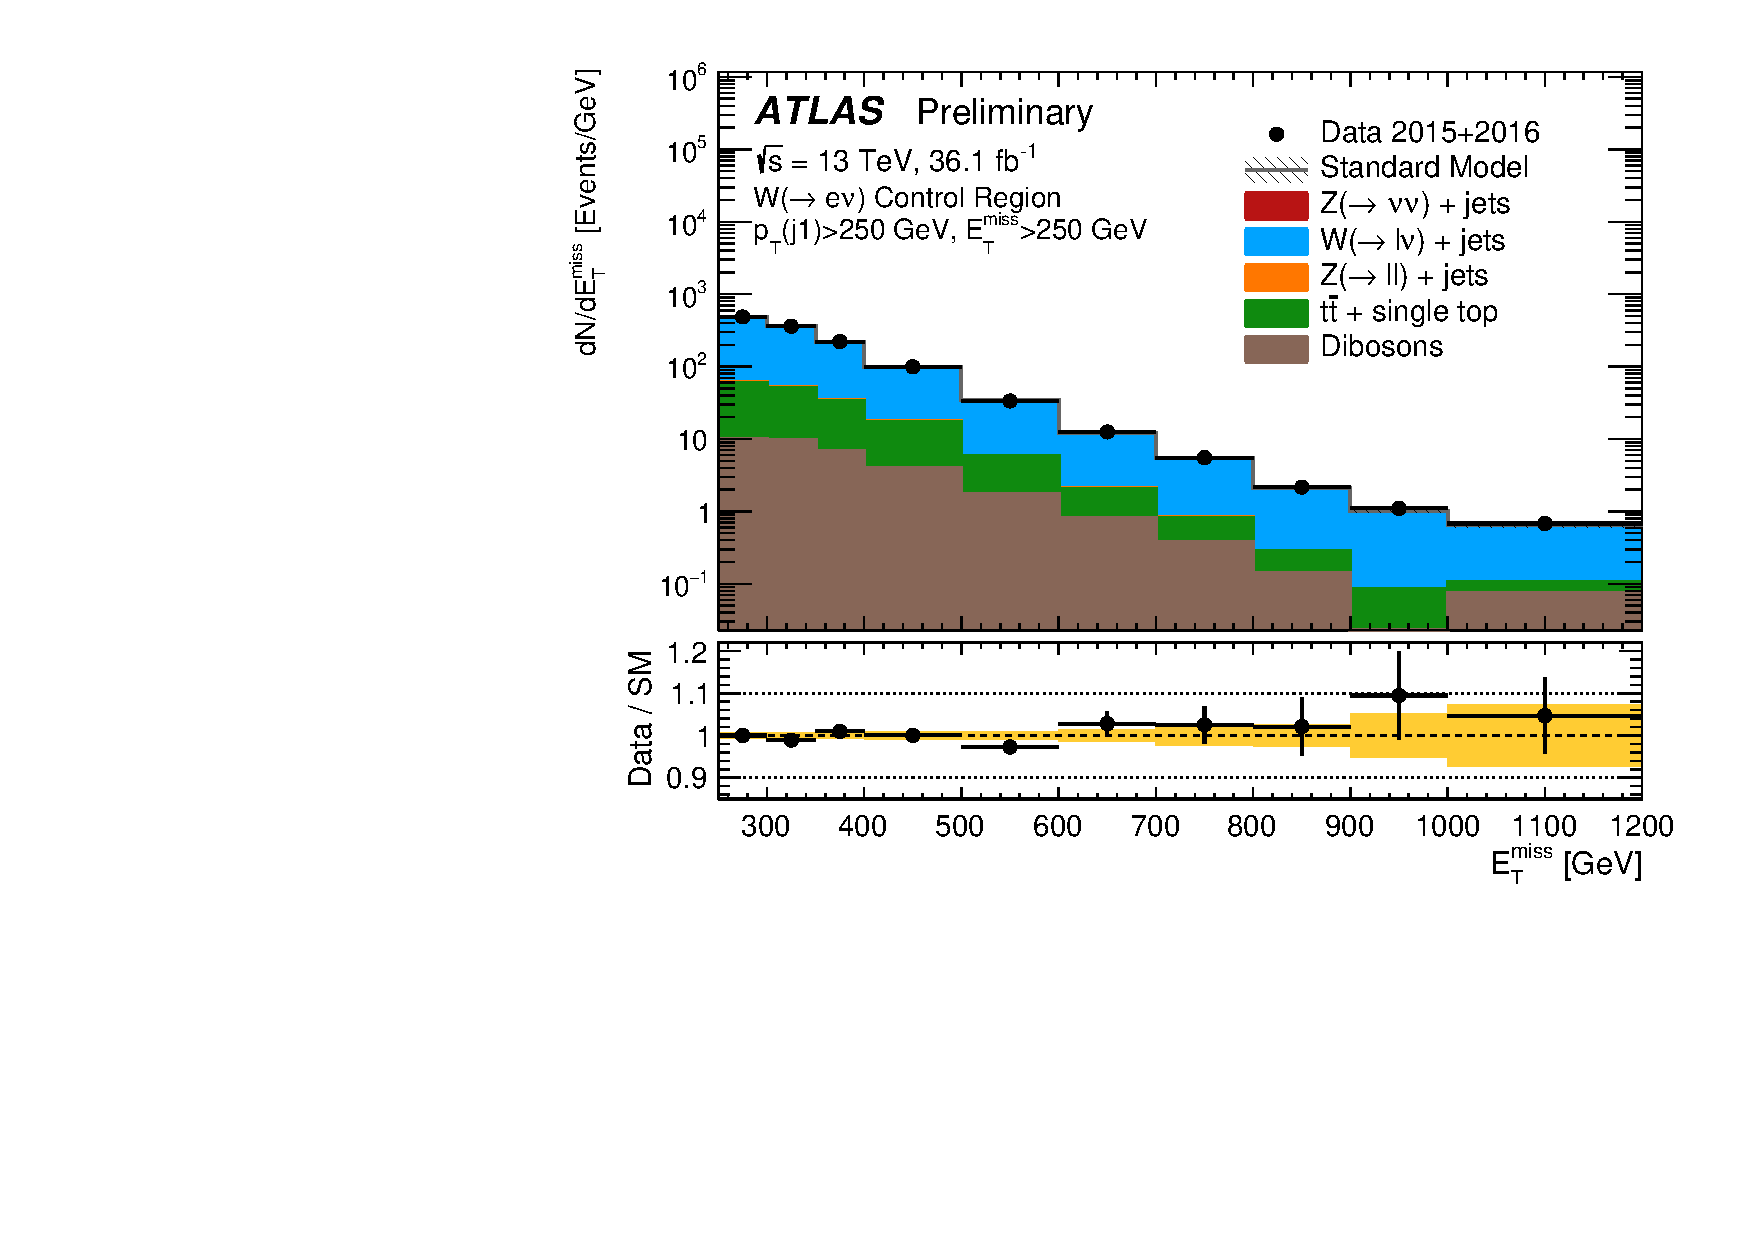
\includegraphics[width=\linewidth]{ele_cr_et_miss_2016}
    \caption{$\met$ distribution.}
    \label{fig:ele_cr_met}
  \end{subfigure}
  \begin{subfigure}[t]{.48\linewidth}
    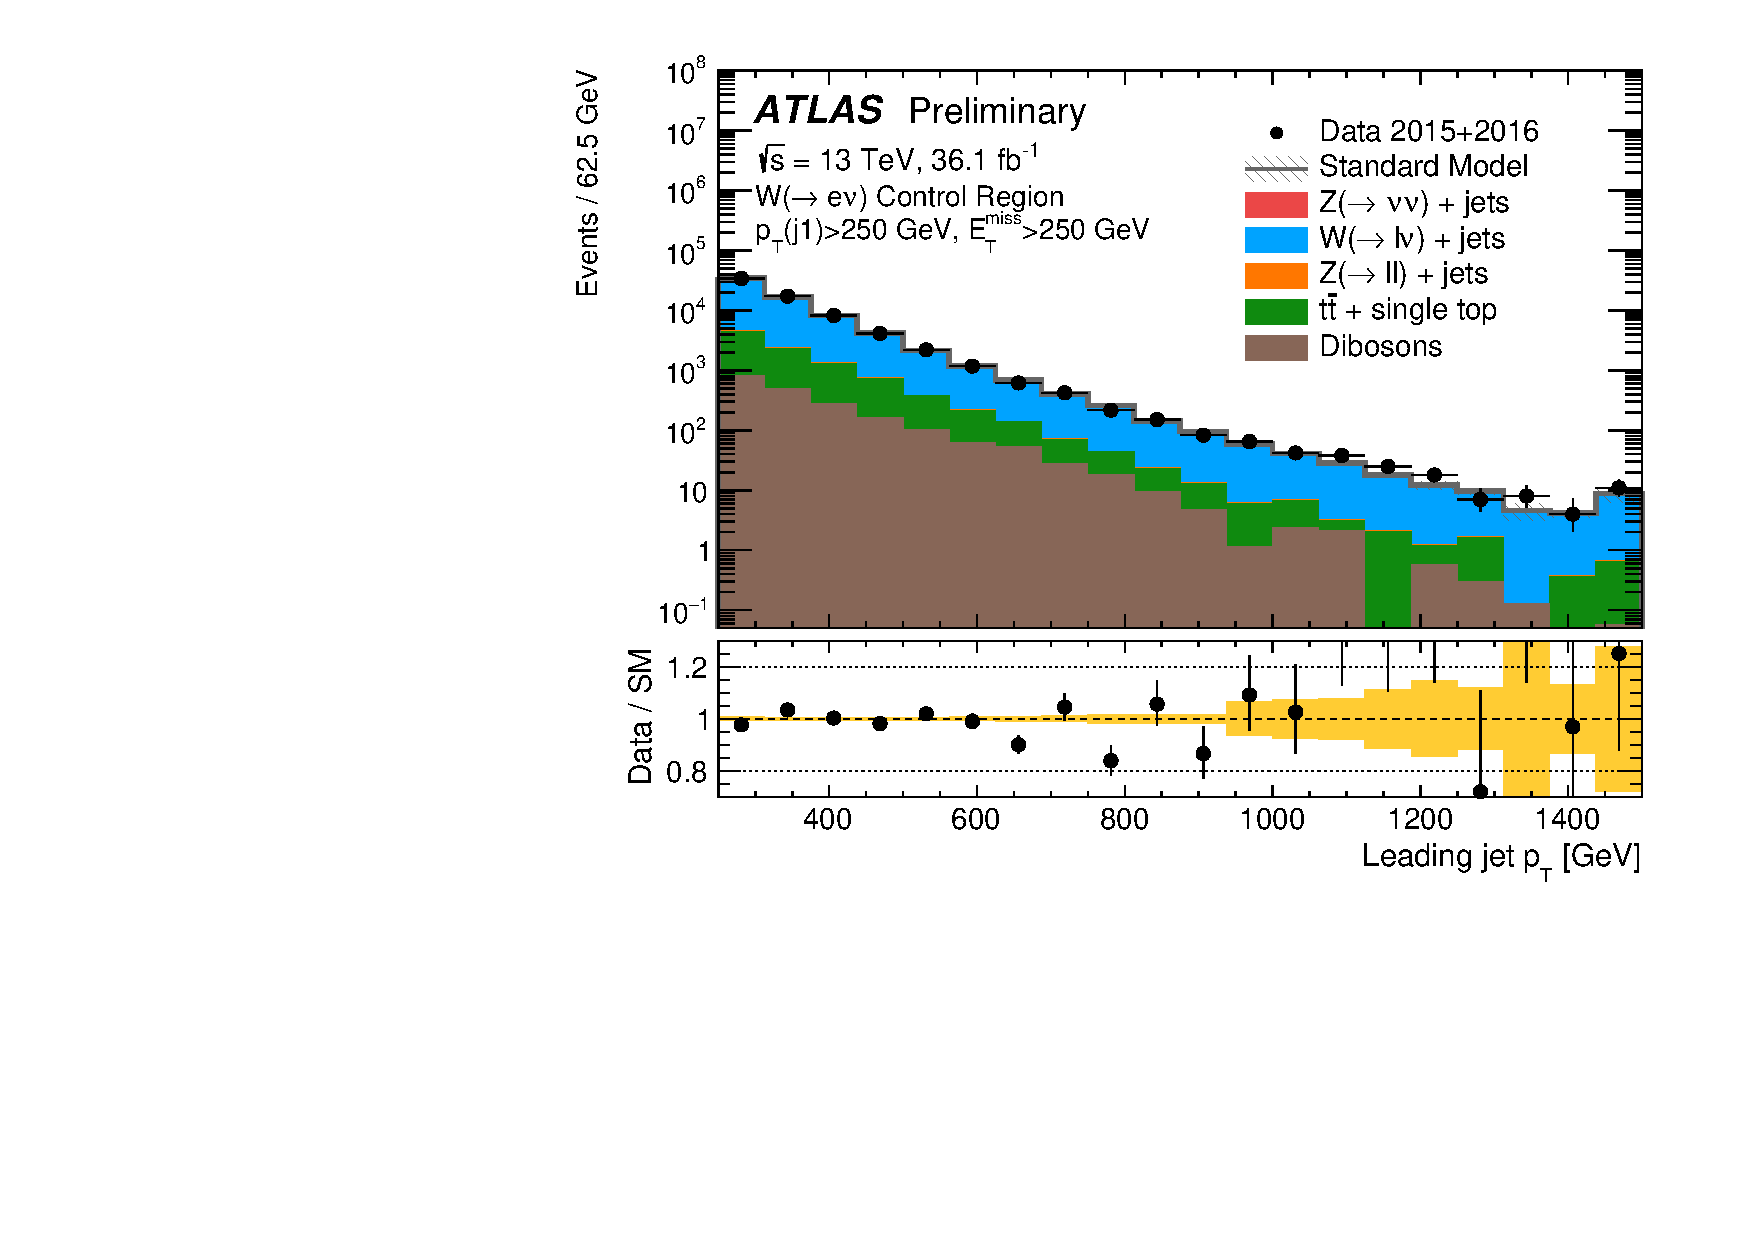
\includegraphics[width=\linewidth]{ele_cr_jet1_2016}
    \caption{Leading jet $\pt$ distribution.}
    \label{fig:ele_cr_jet1}
  \end{subfigure}
  \caption{Observed and predicted $\met$ and leading jet $\pt$ after the
    background only fit in the $\crele$ control region for the $\met > 250$~GeV
    inclusive selection corresponding to IM1. The error bands in the ratio plot
    on the bottom of the figures include statistical and systematic
    uncertainties. The negligible contribution of \gls{ncb} and diboson
    backgrounds is not reported in the figure.}
  \label{fig:ele_cr_plots_2016}
\end{figure}
%%% Local Variables:
%%% mode: latex
%%% TeX-master: "../search_for_DM_LED_with_ATLAS"
%%% End:
